\documentclass[10pt,a4paper]{article}
\usepackage[utf8]{inputenc}
\usepackage[russian]{babel}
\usepackage[OT1]{fontenc}
\usepackage{amsmath}
\usepackage{amsfonts}
\usepackage{amssymb}
\usepackage[dvipsnames]{xcolor}
\usepackage{graphicx}
\graphicspath{{Images/}}
\usepackage[left=2cm,right=2cm,top=2cm,bottom=2cm]{geometry}
\usepackage{calc}
\usepackage{wrapfig}
\usepackage{setspace}
\usepackage{indentfirst}
\usepackage{subfigure}
\usepackage{multirow}
\usepackage{amsfonts}
\usepackage{hyperref}
\hypersetup{
    pdfstartview=FitH,  
    linkcolor=black,
    urlcolor=red, 
    colorlinks=true,
    citecolor=blue}
\usepackage{tikz}
\usetikzlibrary{ decorations.markings}

\title{Семинар 17}
\date{\today}

\author{Варламов Антоний Михайлович}

\begin{document}
		\maketitle

	\section{Исследование многошаговых методов на устойчивость}	
	
	\begin{equation}\label{eq:problem}
		\begin{cases}
			\frac{d{u}}{dt} = {f}\left(u, t\right), \ t\in[0, T]
			\\
			{u}\left(0\right) = {u}_{0}
		\end{cases}
	\end{equation}
	
	Для рассмотрения вопросов устойчивости от задачи (\ref{eq:problem}) можно 
	перейти к уравнению Далквиста, которое выглядит как:
	
	\begin{equation}
			\begin{cases}
				\frac{du}{dt} = \lambda u, \Re\left(\lambda\right) \leqslant 0
				\\
				u\left(0\right) = u_{0}
			\end{cases}
	\end{equation}
	
	Для схем, которые мы исследовали на устойчивость ранее, мы могли явным 
	образом выразить функцию перехода между двумя лагами по времени:
	
	\begin{equation}
		y_{n + 1} = R\left(\lambda\Delta t\right) \cdot y_{n}
	\end{equation}
	
	При этом условие устойчивости: 
	\begin{equation}
		\left|R\left(z\right)\right| \leqslant 1
	\end{equation}
	
	Данное неравенство накладывает ограничения на величину $\Delta t$ при 
	фиксированном значении $\lambda$.
	
	В случае многошаговых методов, получить такую связь между двумя 
	последовательными шагами по времени в общем случае невозможно. Рассмотрим в 
	качестве примера явный метод Адамса второго порядка:
	
	\begin{equation}
		\frac{y_{n + 1} - y_{n}}{\Delta t} = \frac{3}{2}f_{n} - \frac{1}{2}f_{n 
		- 1}
	\end{equation}
	
	Применяя его для решения уравнения Далквиста получаем:
	
	\begin{equation}
		\frac{y_{n + 1} - y_{n}}{\Delta t} = \frac{\lambda}{2}\left(3y_{n} - 
		y_{n - 1}\right)
	\end{equation}

	\begin{equation}
		y_{n + 1} - y_{n}\left(1 + \frac{3}{2}\lambda\cdot\Delta t\right) + 
		\frac{\Delta t \lambda}{2}y_{n - 1}  = 0
	\end{equation}
	
	Решим данное разностное уравнение. Искать решение будем в виде: $y_{n} = 
	\Theta^{n}$.
	
	Получаем:
	
	\begin{equation}
		\Theta^{2} - \Theta\left(1 + \frac{3}{1}z\right) + \frac{z}{2} = 0
	\end{equation}
	
	Откуда получаем значения $\Theta_{1, 2}$ для корней 
	\textit{характеристического многочлена}. 
	
	Общее решение будет выглядеть следующим образом:
	
	\begin{align}
		y_{n} &= C_{1}\Theta_{1}^{n} + C_{2}\Theta^{n}_{2}, \ \text{в случае 
		простых корней,}\\
	 	y_{n} &= C_{1}\Theta^{n} + C_{2}n\Theta^{n}, \ \text{если корень 
	 	кратный.}
	\end{align}
	
	Тогда для ограниченности численного решения мы должны потребовать:
	
	\begin{align}
		\left|\Theta_{1, 2}\right|& \leqslant 1 - \text{простые корни,} \\
		\left|\Theta\right|& < 1 - \text{кратные корни.}
	\end{align}
	
	Однако, производить оценку модуля корней может быть довольно затруднительно, 
	поэтому есть альтернативный вариант. Будем искать \textit{границу области 
	устойчивости} исследуемого метода:
	
	\begin{equation}
		\frac{z}{2} - \frac{3}{2}z\Theta = \Theta - \Theta^{2}
	\end{equation}
	
	\begin{equation}
		z\left(\frac{1}{2} - \frac{3}{2}\Theta\right) = \Theta\left(1 - \Theta
		\right)
	\end{equation}
	
	\begin{equation}
		z = \frac{\Theta\left(1 - \Theta\right)}{\frac{1}{2} - \frac{3}{2}
		\Theta}
	\end{equation}
	
	Для точек границы области устойчивости должно выполняться:
	
	\begin{equation}
		\left|\Theta\right| = 1
	\end{equation}
	
	Значит, $\Theta  = e^{i\varphi}, \varphi \in \left[0, 2\pi\right]$
	
	\begin{equation}
		z = \frac{e^{i\varphi}\left(1 - e^{i\varphi}\right)}{\frac{1}{2} - 
		\frac{3}{2}e^{i\varphi}}
	\end{equation}
	
	Таким образом, мы получили явное выражение $z(\varphi)$.
	
	\begin{figure}[h!]
		\centering
		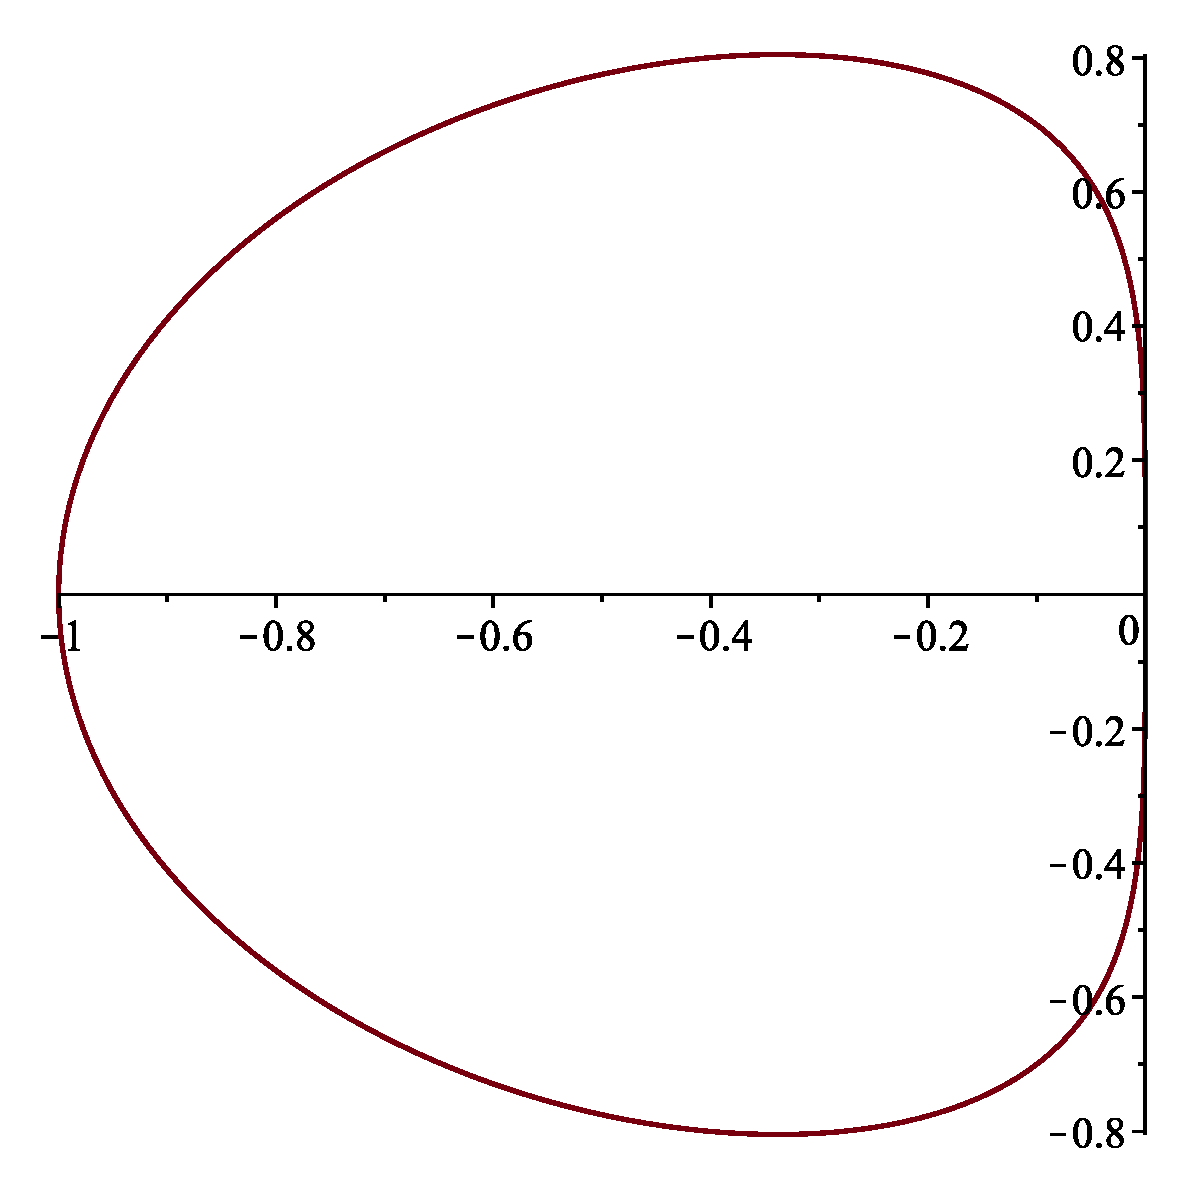
\includegraphics[width = 0.5\linewidth,keepaspectratio]
		{Zone_boarder.eps}
		\caption{Граница области устойчивости в комплексной плоскости,
	 	определяемая выражением 
		$z = \frac{e^{i\varphi}\left(1 - e^{i\varphi}\right)}{\frac{1}{2} - 
		\frac{3}{2}e^{i\varphi}}$}
	\end{figure}
	
	Перейдем к рассмотрению устойчивости решения систем ОДУ:
	
	\begin{equation}
		\frac{d\vec{u}}{dt} = A\cdot\vec{u}
	\end{equation}
	
	Для простоты воспользуемся явным методом Эйлера:
	
	\begin{equation}
		\frac{\vec{y}_{n + 1} - \vec{y}_{n}}{\Delta t} = A\vec{y}_{n}
	\end{equation}
	
	Выражаем:
	
	\begin{equation}
		\vec{y}_{n + 1} = \left(I + \Delta t\cdot A\right)\cdot 
		\vec{y}_{n} \equiv S \cdot  \vec{y}_{n}
	\end{equation}
	
	\begin{equation}
		\parallel \vec{y}_{n + 1}\parallel \leqslant \parallel\vec{y}_{n}
		\parallel
	\end{equation}
	
	Рассмотрим конкретный пример:
	
	\begin{equation}
		A = \begin{pmatrix}
			98 & 198\\
			-99 & -199
		\end{pmatrix}
	\end{equation}
	
	\begin{equation}
		\vec{y}_{n + 1} = \begin{pmatrix}
			1+98 \Delta t & 198\Delta t\\
			-99\Delta t & 1-199\Delta t
		\end{pmatrix}
		\cdot\vec{y}_{n}
	\end{equation}
	
	Для решения такой системы разностных уравнений необходимо рассмотреть 
	выражение:
	
	\begin{equation}
		\lambda\left(S\right) = 1 + \Delta t\lambda\left(A\right) 
	\end{equation}
	
	\begin{equation}
		\begin{cases}
			\lambda_{1}\left(A\right) = -1
			\\
			\lambda_{2}\left(A\right) = -100
		\end{cases}
	\end{equation}
	
	Для данный собственных чисел определяем собственные вектора:
	
	\begin{equation}
		\begin{cases}
			\vec{v}_{\lambda_{1}\left(A\right)} = \begin{pmatrix}
			-2\\1
			\end{pmatrix}
			\\
			\vec{v}_{\lambda_{2}\left(A\right)} = \begin{pmatrix}
			-1\\1
			\end{pmatrix}
		\end{cases}
	\end{equation}
	
	Тогда общее решение записывается в виде:
	
	\begin{equation}
		\vec{y}_{n} = C_{1}\begin{pmatrix}
			-2\\1
			\end{pmatrix} \left(1 - \Delta t\right)^{n} + 
			C_{2} \begin{pmatrix}
			-1\\1
			\end{pmatrix}\left(1 - 100\Delta t\right)^{n}
	\end{equation}
	
	Для ограниченности такого решения нужно потребовать:
	
	\begin{equation}
		\begin{cases}
			\left|1 + \lambda_{1}\Delta t\right| \leqslant 1
			\\
			\left|1 + \lambda_{2}\Delta t\right| \leqslant 1
		\end{cases}
	\end{equation}
	
	\begin{equation}
		\begin{cases}
			\left|1 - \Delta t\right| \leqslant 1
			\\
			\left|1 - 100\Delta t\right| \leqslant 1
		\end{cases}
	\end{equation}
	
	Данная система сводится к:
	
	\begin{equation}
		\begin{cases}
			\Delta t\leqslant 2
			\\
			\Delta t \leqslant \frac{1}{50}
		\end{cases}
		\Rightarrow \Delta t \leqslant \frac{1}{50}
	\end{equation}
	
	Вид ограничений, который мы получили, совпадает со случаем применения явного 
	метода Эйлера для уравнения Далквиста, где в качестве $\lambda$ используется 
	собственные значения матрицы $A$. 
	
	Рассмотрим еще один пример:
	
	\begin{equation}
		\begin{cases}
			\frac{d^{2}u}{dt^{2}} + \omega^{2}u = 0
			\\
			u\left(0\right) = u_{0}
			\\
			u'\left(0\right) = 0
		\end{cases}
	\end{equation}
	
	От данной системы перейдем к ОДУ вида:
	
	\begin{equation}
		\begin{cases}
			\frac{du}{dt} = v
			\\
			\frac{dv}{dt} = -\omega^{2}u
			\\
			u\left(0\right) = u_{0}
			\\
			v\left(0\right) = 0
		\end{cases}
	\end{equation}
	
	Исследуем на устойчивость явный метод Эйлера для решения этой системы:
	
	\begin{equation}
		\begin{cases}
			\frac{u_{n + 1} - u_{n}}{\Delta t} = v_{n}
			\\
			\frac{v_{n + 1} - v_{n}}{\Delta t} = -\omega^{2}u_{n}
		\end{cases} \Rightarrow A = \begin{pmatrix}
			0	&	 1 \\
			-\omega^{2} & 0
		\end{pmatrix}
	\end{equation}
	
	\begin{equation}
		\lambda^{2} + \omega^{2} = 0 \Rightarrow \lambda_{1,2} = \pm i\omega
	\end{equation}
	
	Из условия устойчивости:
	
	\begin{equation}
		\left|1 - z\right| \leqslant 1
	\end{equation}
	
	Получаем, что 
	
	\begin{equation}
		\left|1 - \Delta t\cdot i\omega\right| \nleqslant 1
	\end{equation}
	
	Т.е. данный метод не является устойчивым.
	
	Для общего случая:
	
	\begin{equation}
		\frac{d\vec{u}}{dt} = F\left(\vec{u}, t\right)
	\end{equation}
	
	Необходимо найти матрицу Якоби $J\left(F\right)$, а затем определить спектр
	данной матрицы, после чего перейти к исследованию устойчивости схемы для 
	уравнения Далквиста:
	
	\begin{align}
		\frac{du}{dt} &= \lambda u,\\
		u(0&)=u_0,
	\end{align}
	 где в качестве $\lambda$ нужно использовать собственные значения матрицы 
	 Якоби.
	
	Рассмотрим пример:
	
	\begin{equation}
		\frac{du}{dt} = -u^{2} \Rightarrow J = -2u
	\end{equation}
	
	Для такого уравнения "спектр матрицы Якоби" зависит от времени. То есть 
	условие на шаг по времени $\Delta t$ может меняться. Учитывая, что при 
	устойчивом счете величина решения не должна возрастать, максимальное 
	значение решения достигается в начальный момент времени. То есть при 
	исследовании устойчивости разностной схемы в качестве значения $\lambda$ в 
	уравнении Далквиста можно использовать $-2 u_0$.  
	
	Воспользуемся явным методом Эйлера для решения этого уравнения:
	
	\begin{equation}
		\frac{y_{n + 1} - y_{n}}{\Delta t} = -y_{n}^{2}
	\end{equation}
	
	Условие устойчивости
	
	\begin{equation}
		\left|1 + \Delta t\left(-2u_0\right)\right| \leqslant 1
	\end{equation}
	
	Приходим к оценке:
	
	\begin{equation}
		\Delta t\leqslant 
		\frac{1}{\left|u_{0}\right|}
	\end{equation}
\end{document}